
\section{PAZZOIDE}
qui spiega.

\section{Componenti}

Ogni plugin per Kibana è articolato in due sezioni principali: lato client e lato server. Si presenta di seguito il dettaglio di ciasuna sezione.

\subsection{Lato Server}
Il lato server si deve occupare di interrogare il database Elasticsearch ed esporre i risultati delle query tramite API REST al lato client.
\subsubsection{Rappresentazione}
Nel seguente diagramma delle classi, figura \ref{img:diagrammaClassiServer}, ciascuna API viene rappresentata tramite una classe composta da un singolo metodo. Tale metodo intende rappresentare il funzionamento della API.


\begin{figure}[h]
	\centering
	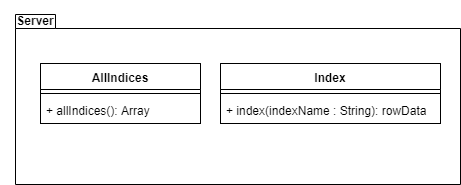
\includegraphics[width=1\textwidth]{Images/DiagrammaClassiServer.png}
	\caption{Diagramma UML delle classi riguardanti il lato server}
	\label{img:diagrammaClassiServer}
\end{figure}

\subsubsection{AllIndices}
AllIndices è la API che si occupa di restituire al chiamante la lista di \emph{tutti} gli indici presenti all'interno della istanza di Elasticsearch collegata. La lista degli indici è un array di stringhe contenente per ogni indice il proprio nome.

\subsubsection{Index}
Index è la API che espone l'interfaccia per poter leggere i dati contenuti all'interno di un indice. Nella richiesta GET deve essere specificato un parametro chiamato index, il cui valore rappresenta l'indice del quale si vogliono ottenere i dati. Ciò che viene ritornato al richiedente è un oggetto \emph{grezzo}, ovvero la risposta dell'istanza Elasticsearch, con tutti i metadati che Elasticsearch utilizza annessi. Sarà compito del client reperire le informazioni a lui utili

\subsection{Lato Client}
Il lato client si occupa di interrogare il lato server per ottenere informazioni grezze, elaborarle per renderle utili ed infine presentarle all'utente.

\label{sec:Componenti}
\subsubsection{Rappresentazione}
Il codice prodotto è stato scritto in Javascript ES6, quindi molti concetti quali classi ed interfacce non sono presenti all'interno del linguaggio. Per produrre un diagramma delle classi dunque sono state considerate \emph{ classi } sia oggetti Javascript, sia funzioni. Per quanto riguarda le interfacce che sono presenti nel diagramma delle classi, figura \ref{img:diagrammaClassiClient}, nel codice non sono effettivamente presenti tali interfacce, ma tutte le classi che implementano tale interfaccia \emph{devono} possedere i metodi esposti da tale interfaccia. Questo stratagemma è stato particolarmente utile nell'implementazione del componente \texttt{DataCleaner}, come descritto in \ref{sec:DataCleaner}

\begin{figure}[H]
    \centering
    
\includegraphics[width=1\textwidth]{Images/logo.jpg}
    \caption{Diagramma delle classi dell'applicazione}
    \label{img:diagrammaClassiClient}
\end{figure}

\subsubsection{DataReader}
\label{sec:DataReader}
\texttt{DataReader} è il componente del sistema che si occupa di reperire i dati da Elasticsearch, interagendo con il lato server. Restituirà ai richiedenti le informazioni grezze, esattamente come vengono restituite da Elasticsearch. I metodi sono:

\begin{itemize}
	\item \texttt{setElasticsearchClient(client)}: permette di impostare una sorgente dei dati;
	\item \texttt{tracesIndices()}: ritorna un array di stringhe, i quali elementi sono tutti e soli gli indici all'interno dell'istanza di Elasticsearch che hanno al loro interno delle traces. Ciò viene realizzato tramite una chiamata al lato server all'API \texttt{AllIndices} e dunque vengono tenuti solo indici che contengono nel nome la sottostringa \emph{spans};
	\item \texttt{readIndex(index)}: ritorna al chiamante i dati grezzi che vengono restituiti da Elasticsearch eseguendo una ricerca priva di parametri sull'indice passato come parametro, ovvero \texttt{index}. Essi comprendono oltre tutti i documenti dell'indice anche i metadati di Elasticsearch;
	\item \texttt{readData()}: ritorna al chiamante un array di dati grezzi, ognuno dei quali rappresenta il risultato di una ricerca priva di parametri su un indice. Gli indici letti sono quelli ritornati da \texttt{tracesIndices()}, ovvero tutti e soli quelli che contengono traces.


\end{itemize}



\subsubsection{DataCleaner}
\label{sec:DataCleaner}
\texttt{DataCleaner} è il componente del sistema che si occupa di pulire i dati grezzi che sono stati reperiti da ElasticSearch. Esso compie questo lavoro in due momenti: prima estraendo i dati "utili" da Elasticsearch e poi pulendoli attraverso una \emph{strategy}, descritta in \ref{sec:CleanerStrategy}.\\
Il metodo \texttt{clean(data)} si occupa di realizzare ciò.
Per estrarre i dati utili esso si avvale di un metodo, \texttt{removeMetaData(data)}, il quale si occupa di rimuovere i metadati di Elasticsearch che sono presenti quando si prelevano i dati. Questo metodo ritorna un array contenente i documenti JSON così come essi sono stati inseriti dall'applicazioni di monitoring negli indici di ElasticSearch. ElasticSearch, infatti, immagazzina i documenti JSON nel campo \texttt{\_source} il quale è inserito in oggetti che contengono altri dati ed informazioni "di servizio". Il metodo si occupa di rimuovere questi dati e costruisce un array contenente il solo contenuto dei campi \texttt{\_source}. Il client che utilizza questa classe comunque in generale ha la necessità di ripulire ulteriormente i dati dei documenti, per esempio eliminando certi tipi di trace (ad esempio tenere solamente traces di richieste HTTP). Per poter soddisfare ogni richiesta specifica un \texttt{DataCleaner} contiene un oggetto che rispetti l'interfaccia \texttt{CleanerStrategy}. La strategy viene incaricata di raffinare ulteriormente i dati per la costruzione della Mappa Topologica oppure per la costruzione dello Stack Trace tramite il metodo \texttt{clean(data)}. \\
Risulta chiaro che esiste dunque una dipendenza fra la struttura dei dati che vengono restituiti da ElasticSearch, la classe \texttt{DataCleaner} e le classi che implementano \texttt{CleanerStrategy}. Tuttavia, i client di \texttt{DataCleaner} potranno avere accesso diretto ai dati di ElasticSearch, privi di dati amministrativi.

	
\subsubsection{CleanerStrategy}
\label{sec:CleanerStrategy}

\texttt{CleanerStrategy} è l'interfaccia che verrà implementata per realizzare una pulizia più raffinata dei dati di un \texttt{DataCleaner}. Espone il metodo \texttt{clean(data)}, che avrà comportamenti diversi a seconda della strategia che si desidera applicare. Dato che il prodotto è implementato in Javascript il costrutto interfaccia non è presente nel linguaggio. Per ovviare a questa mancanza tutte le classi che dovrebbero implementare questa interfaccia \emph{devono} possedere un metodo \texttt{clean(data)} che funzioni come ci si aspetti. 

	
	
\subsubsection{GraphCleaner}
\label{sec:GraphCleaner}

\texttt{GraphCleaner} è l'implementazione di \texttt{CleanerStrategy} utilizzata da \texttt{DataCleaner} per pulire i dati che dovranno essere utilizzati per la costruzione del grafo rappresentante la mappa topologica. Essa implementa il metodo \texttt{clean(data)} il quale scorre tutti i documenti JSON disponibili e ha come output esclusivamente l'insieme di questi documenti che rappresentano richieste di dati ai database dell'applicazione oppure a server, ovvero il sottoinsieme di quelle che serviranno per la costruzione del grafo.
	
\subsubsection{StackCleaner}
\label{sec:StackCleaner}

\texttt{StackCleaner} è l'implementazione di \texttt{CleanerStrategy} utilizzata da \texttt{DataCleaner} per pulire i dati che dovranno essere utilizzati durante la costruzione della stack trace. Essa dispone del metodo \texttt{clean(data)} il quale scorre tutti i documenti JSON disponibili e ha come output l'insieme di documenti che rappresentano chiamate HTTP, JDBC oppure Pageload, ovvero tutte e sole quelle necessarie per la costruzione dei dati strutturati della stack trace.



\subsubsection{StackBuilder}
\label{sec:StackBuilder}

\texttt{StackBuilder} si occupa della riorganizzazione dei dati e della loro elaborazione in modo da ottenere una struttura dati ottimale per la successiva visualizzazione della Stack Trace.\\
Esso viene istanziato con un oggetto \texttt{DataReader} per poter ottenere i dati.
Il metodo principale è \texttt{getStack()} che controlla tutte le chiamate HTTP ricevute dal \texttt{DataReader} e pulite dal \texttt{DataCleaner}, creato e istanziato con strategia \texttt{StackCleaner}. \texttt{GetStack()} riorganizza i dati in base alla loro tipologia per poter essere successivamente mostrati in modo più agevole. Essi possono essere di tre tipi:
	\begin{itemize}
		\item HTTP: insieme di metodi scatenati da un evento generico;
		\item HTTP + Pageload: insieme di metodi scatenati dal caricamento di una pagina web;
		\item HTTP + JDBC + Pageload: insieme di eventi che portano all'interrogazione di un database e che provocano un successivo caricamento di una pagina.
	\end{itemize}
	Per ognuna di queste tipologie è costruita una struttura dati che seleziona solo i campi del JSON ricevuto da \texttt{StackCleaner()} veramente utili alla generazione della stack trace. Per ognuna deve essere presente:
	\begin{itemize}
		\item \texttt{type}: che riconduce ad una delle tre tipologie di trace;
		\item \texttt{trace\_id}: numero univoco che permette l'associazione tra trace HTTP, JDBC e Pageload;
		\item \texttt{name}: identificazione generale della richiesta;
		\item \texttt{call\_tree}: array contenente gerarchicamente la lista dei metodi invocati dall'applicazione per compiere la richiesta;
		\item \texttt{duration}: tempo impiegato dal sistema per lo svolgimento della richiesta, compreso il tempo dei metodi, delle query e del caricamento della pagina;
		\item \texttt{timestamp}: data e ora dello svolgimento della richiesta;
		\item \texttt{error}: presenza o meno di errori;
		\item \texttt{status\_code}: tipologia di errore.
	\end{itemize}
	In particolare per il campo \texttt{call\_tree} avviene un'accurata manipolazione del dato attraverso i metodi \texttt{build\_tree()} e \texttt{tableTOtree()}. Al primo metodo viene  passato il dato sotto forma di stringa in cui, attraverso l'ASCII art, viene rappresentato un albero dei metodi che vengono invocati con delle informazioni particolari per ognuno di essi. Questo metodo costruisce un array bidimensionale che elenca tutti i metodi e per ognuno ne specifica i dati aggiuntivi rappresentati dall'ASCII art (come total time e self time), il grado di indentazione nell'albero, il numero di metodi figli e il numero di metodi discendenti da esso. \\ Da questa struttura il metodo \texttt{tableTOtree()} ricava un oggetto con innestati altri oggetti rappresentanti i metodi e i propri dati strutturati in maniera da rispecchiare i legami di parentela dell'ASCII art.


	\textcolor{red}{QUI LISA DESCRIVI GLI ALTRI METODI PRESENTI}

\subsubsection{GraphBuilder}
\label{sec:GraphBuilder}
	\texttt{GraphBuilder} è il componente che si occupa di costruire il grafo di nodi e archi rappresentanti la mappa topologica dell'applicazione. Esso verrà successivamente visualizzato utilizzando la libreria D3.js. \texttt{GraphBuilder} viene istanziato con un oggetto \texttt{DataReader} per poter ottenere i dati di cui ha bisogno. Il metodo più importante è \texttt{getGraph()} che costruisce il grafo partendo dai dati letti dal \texttt{DataReader}. Quando si invoca tale metodo, viene costruito il \texttt{DataCleaner} con strategia \texttt{GraphCleaner} e i dati grezzi vengono letti e successivamente ripuliti dai relativi componenti.
	I metodi \texttt{getNodes()} e \texttt{getLinks()} vengono utilizzati per poter completare la costruzione del grafo.\\
	Il metodo \texttt{getNodes(data)} costruisce l'insieme di nodi che faranno parte della mappa topologica. Esso scorre tutti i documenti JSON preparati dal \texttt{GraphCleaner} e a seconda della tipologia di chiamata (a Database oppure a Server) crea un candidato ad entrare nella lista e attraverso il metodo \texttt{checkIfNotPresent} si assicura che il candidato non sia già presente nella lista che verrà ritornata.\\
	Il metodo \texttt{getLinks(data)} invece costruisce l'insieme di collegamenti che ci saranno tra i nodi del grafo. Un link tra due nodi è caratterizzato dal campo \texttt{source}, il nodo che ha effettuato la chiamata, il campo \texttt{target}, quello che ha ricevuto la chiamata, il campo \texttt{type} che può essere "Database" o "Server". Il campo \texttt{average\_response\_time} che contiene il tempo medio di risposta tra source e target, infine il campo \texttt{number\_of\_requests} che serve per tenere aggiornato il campo avg resp time. Ogni nodo è individuato univocamente dalla coppia \texttt{source} e \texttt{target}.
	In seguito attraverso il metodo \texttt{checkIfLinkIsNotPresent} viene controllato che la coppia source e target del candidato non sia già contenuta nella lista. Se essa non lo è, il nuovo collegamento viene inserito, se invece è già contenuto si limita ad aggiornare i campi \texttt{average\_response\_time} e \texttt{number\_of\_requests}. 

\section{Visualizzazione delle informazioni}

\subsection{Mappa topologica}

\subsection{StackTrace}


\section{Interazioni fra componenti}
\label{sec:Interazioni}
Qui diagrammi di sequenza

\section{Tracciamento dei requisiti}
\label{sec:Tracciamento}
Qui swego 
